
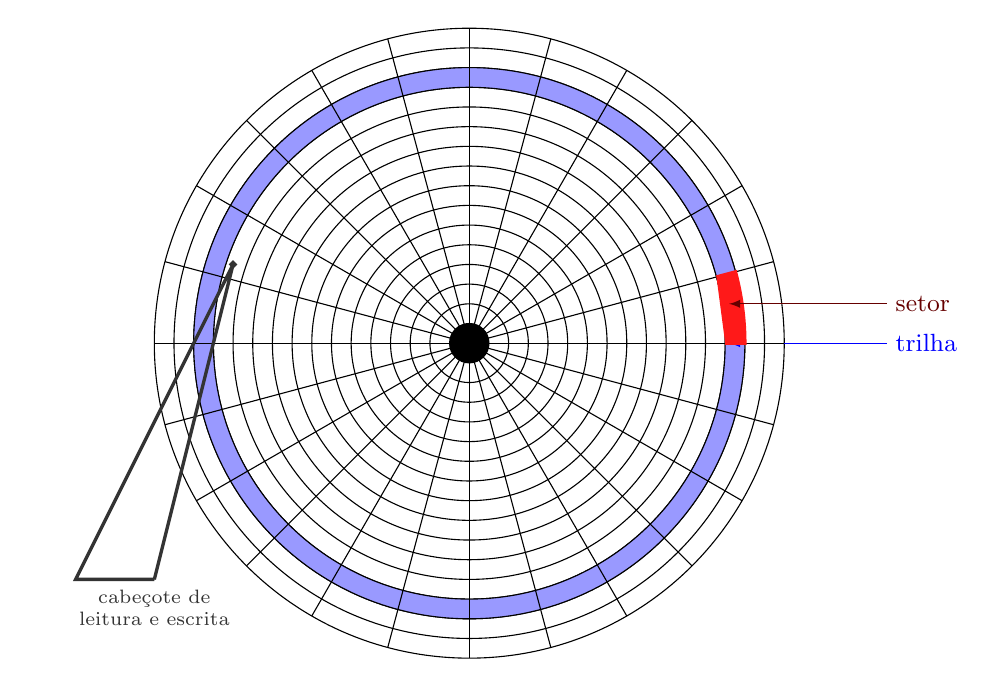
\begin{tikzpicture}\small
  \def\R{4}

  \foreach \d in {0,0.5,1,1.5,...,7} {
    \draw[] (0,0) circle (\R-.5*\d) node (r\d) {};
  }
  \filldraw (0,0) circle (0.25); % AXIS
  \filldraw<1>[even odd rule,fill=blue!40] (0,0) circle (3.5) (0,0) circle (3.25); % TRACK
  \path<1>[blue,draw,<-,>=latex] (3.3,0) -- +(\R/2,0) node[blue,right] {trilha}; % TRACK LABEL
 
  %SECTORS
  \foreach \angle in {0,15,30,...,345}\draw<2-> (0,0) -- +(\angle:\R);
  \filldraw<2>[red!90,very thick] (3.25,0) -- +(.25,0) arc (0:15:3.5) -- +(15:-.25); 
  \path<2>[red!40!black,draw,<-,>=latex] (3.3,0.5) -- +(\R/2,0) node[right] {setor};
 
  %%HEAD
  \path<3>[black!80,draw,very thick] (-4,-3) -- +(1,4) 
  circle (.025) -- +(-1,0) -- (-4,-3) 
  node[font=\scriptsize,text width=3cm,text centered,below] {cabeçote de leitura e escrita}; 

\end{tikzpicture}